\documentclass{article}
\usepackage[utf8]{inputenc}
\usepackage[ngerman]{babel}
\usepackage{pmboxdraw}

% Convenience improvements
\usepackage{csquotes}
\usepackage{enumitem}
\usepackage{amsmath}
\usepackage{amssymb}
\usepackage{mathtools}
\usepackage{tabularx}

% Proper tables and centering for overfull ones
\usepackage{booktabs}
\usepackage{adjustbox}

% Change page/text dimensions, the package defaults work fine
\usepackage{geometry}

\usepackage{parskip}

\usepackage{listings}

% Drawings
\usepackage{tikz}

% Adjust header and footer
\usepackage{fancyhdr}
\pagestyle{fancy}
\fancyhead[L]{Betriebssysteme --- \textbf{Übung 4}}
\fancyhead[R]{Laurenz Weixlbaumer (11804751)}
\fancyfoot[C]{}
\fancyfoot[R]{\thepage}
% Stop fancyhdr complaints
\setlength{\headheight}{12.5pt}

\newcommand{\R}{\mathbb{R}\ \\\ \{0\}}

\newcommand{\cmod}{\text{mod}}

\newcommand{\bO}{\text{O}}

\begin{document}

\begin{enumerate}
    \item Die Positionen der Partitionstabellen ergeben sich aus \enquote{mmls /dev/sdb}, die Form und Eintr\"age aus dem Dump der jeweiligen Tabellen (etwa durch \enquote{dd if=/dev/sdb bs=512 count=1 2>/dev/null | hd}). Dadurch l\"asst sich auch extended/nicht extended anhand der Existenz entsprechender extended Tables erkennen.
    
    Position und Gr\"o{\ss}e der Partitionen und nicht-allokierten Bereiche l\"asst sich gut aus \enquote{mmls /dev/sdb} und \enquote{fdisk -l /dev/sdb} ablesen. Das jeweilige Device-File l\"asst sich in \enquote{gparted} ablesen.
    
    \begin{center}
        \makebox[0pt]{
            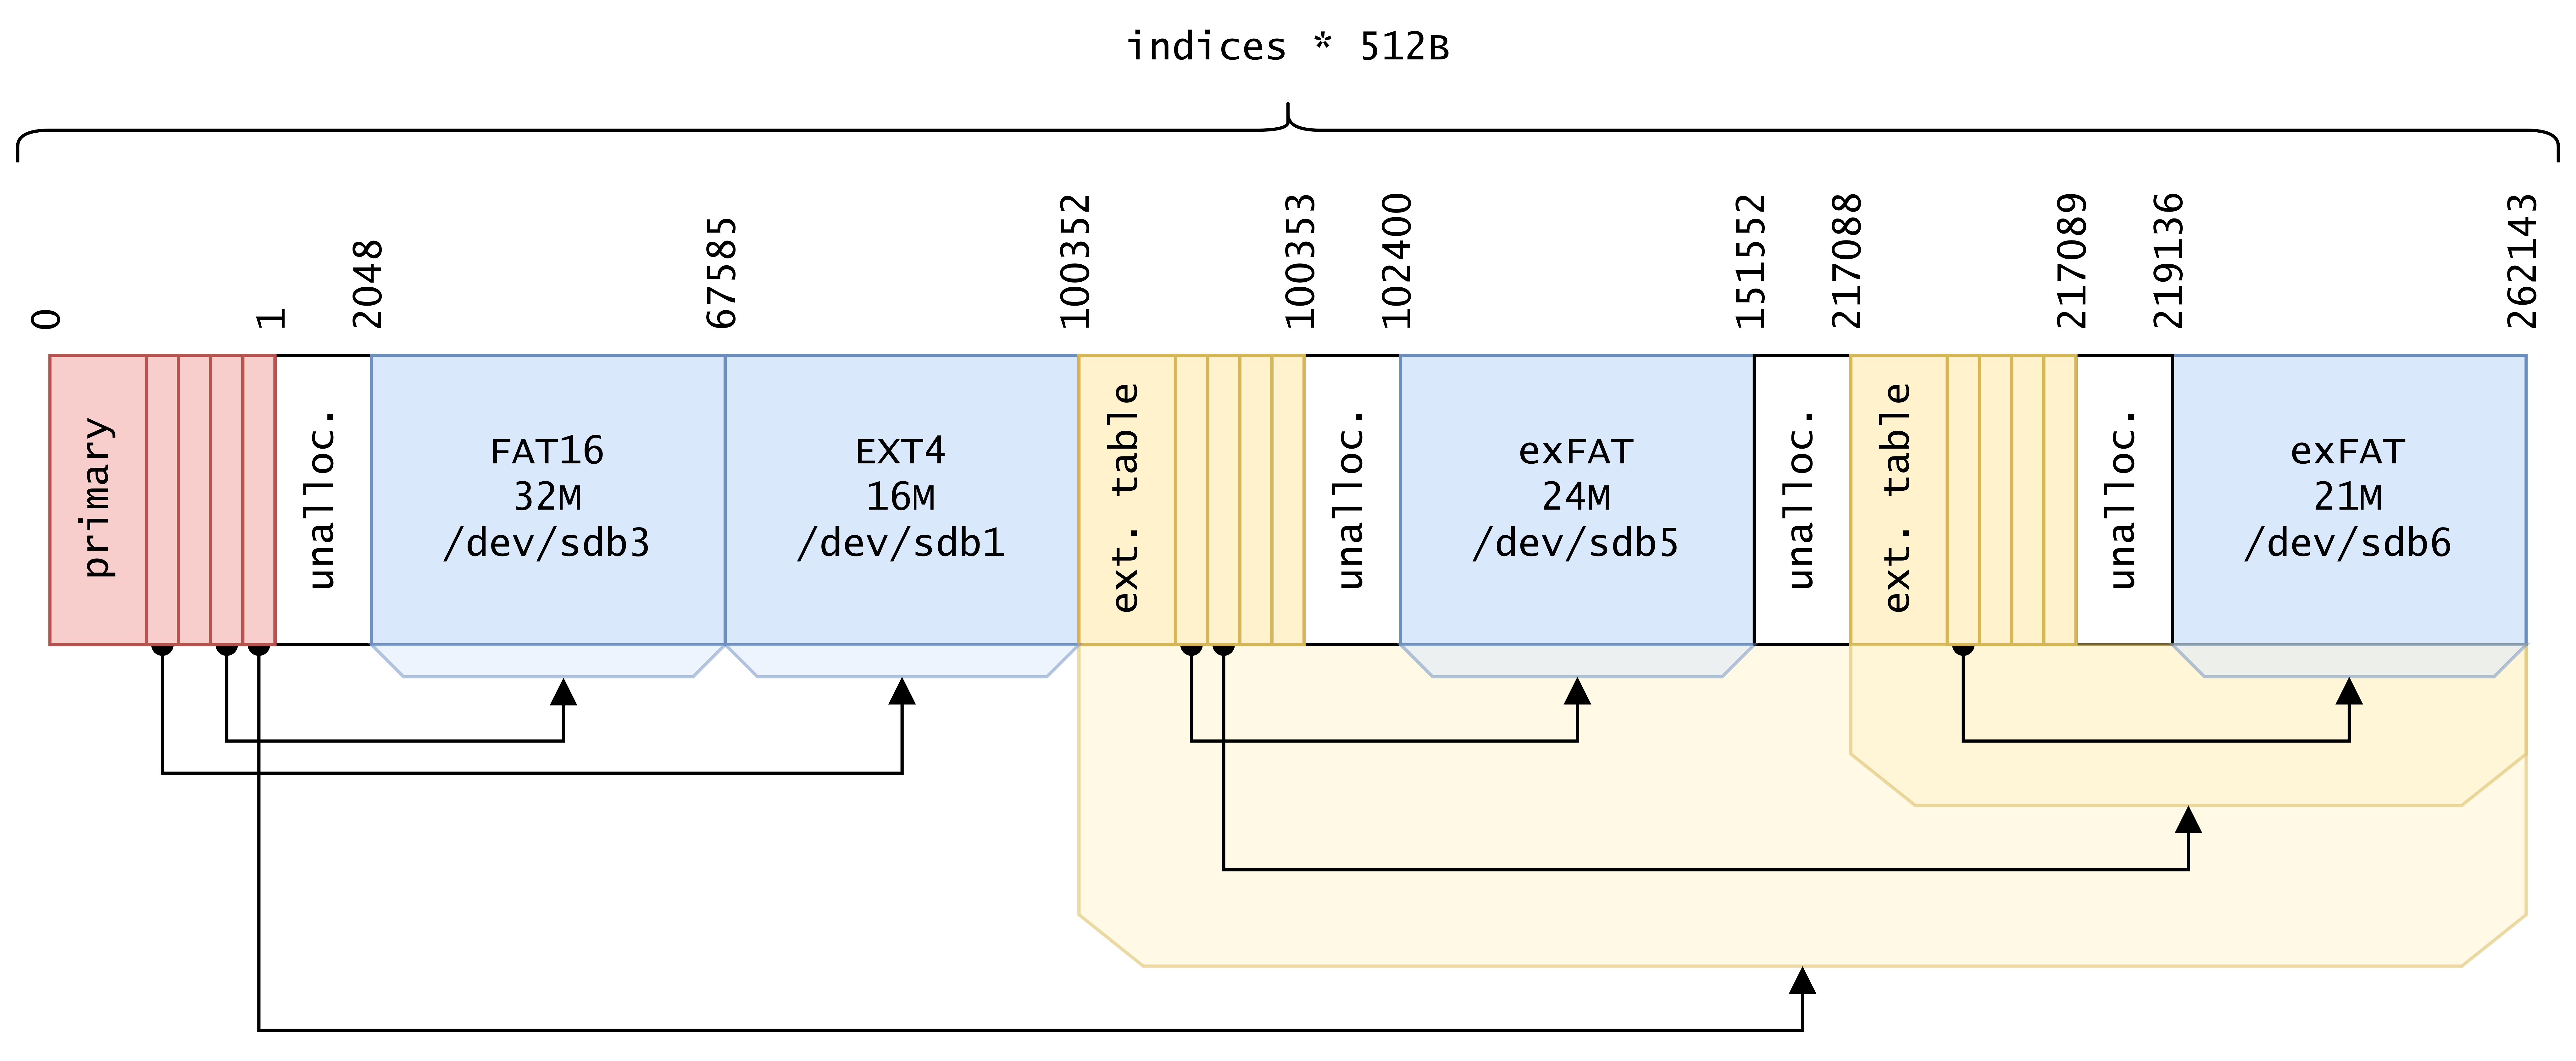
\includegraphics[width=1.25\textwidth]{layout.png}
        }
    \end{center}

    \item \begin{description}
        \item[sdb1] L\"asst sich mounten. 14M frei, 273K belegt.
        \begin{verbatim}
.
├── [     12]  dir002                    # directory
│   └── [     19]  test.dat              # regular file
├── [     13]  dir003                    # regular file
├── [   2049]  dir123                    # directory
├── [     15]  file001 -> dir002/test.dat   # symlink to file
├── [   2050]  interesting                  # directory
│   ├── [     13]  and_another_file         # regular file
│   ├── [     16]  a_special_file -> ../dir002  # symlink to directory
│   └── [   2051]  something_weird              # directory
                       # symlink to parent of parent (yes we are)
│       └── [     18]  are_we_running_in_circles -> ../../interesting 
               # directory with rwx------ permissions, only owner (root) can do anything 
├── [     11]  lost+found [error opening dir]
               # symlink to a directory outside the partition
└── [     14]  what_is_this -> /etc/default
        \end{verbatim}

        Kein echter Baum, es gibt einen geschlossenen Pfad (are\_we\_running\_in\_circles zu interesting).
        \begin{center}
            \makebox[0pt]{
            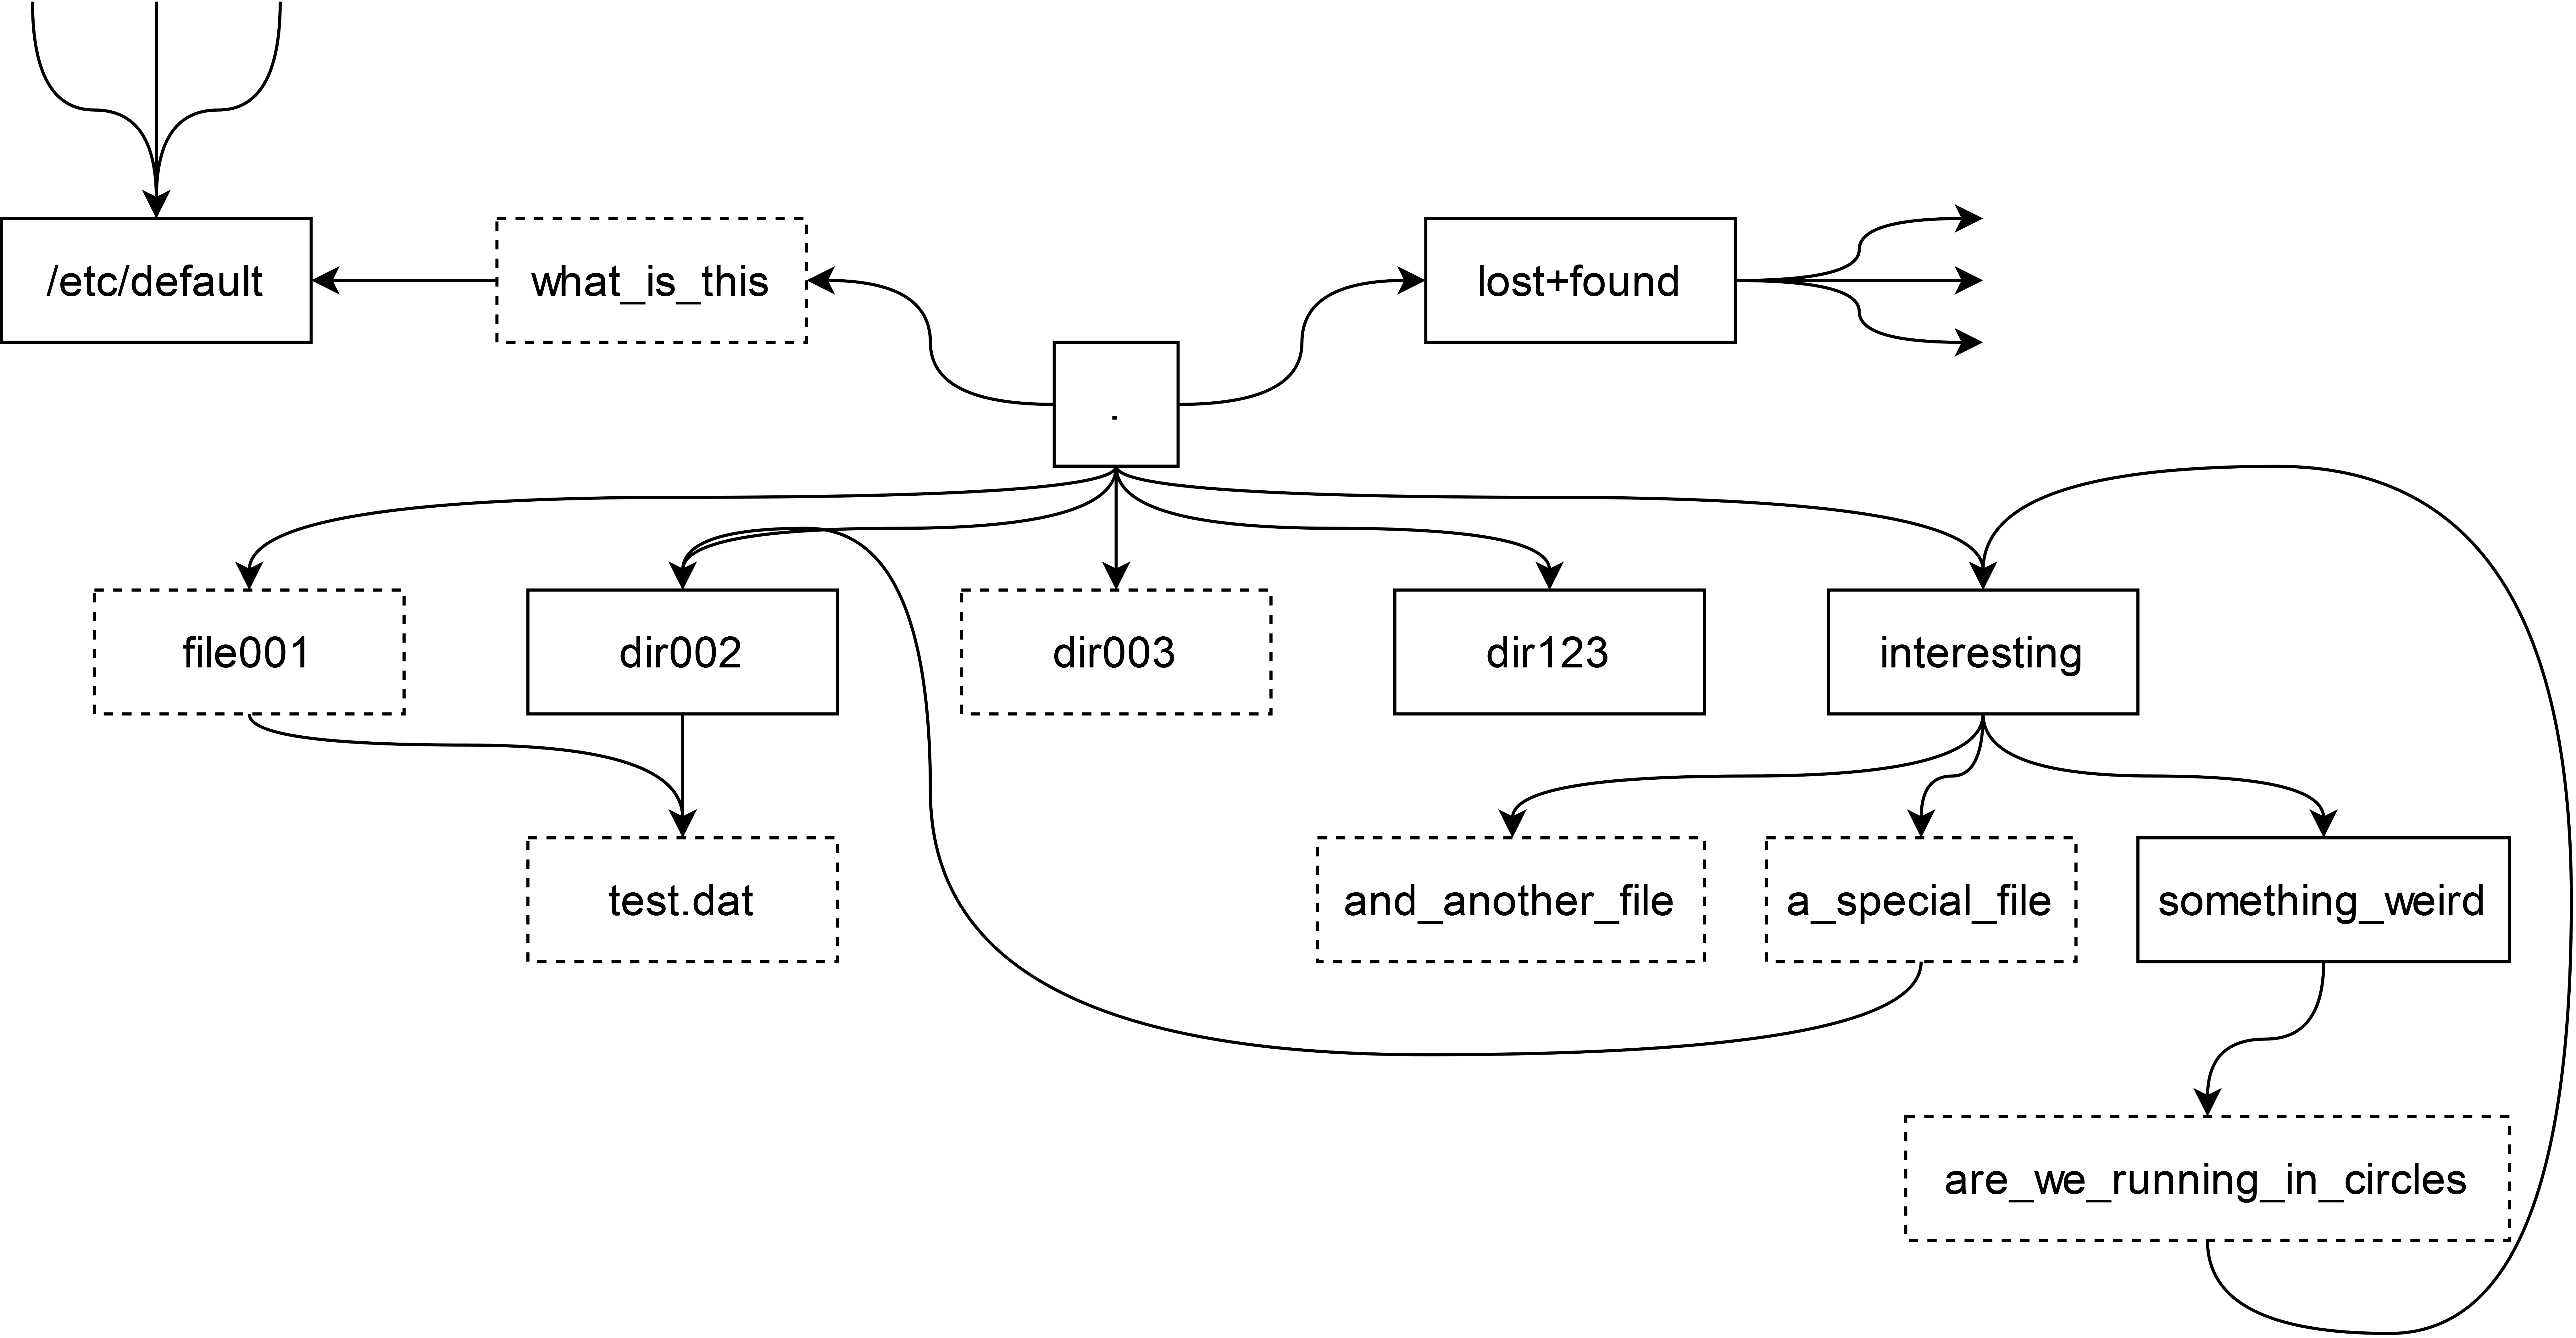
\includegraphics[width=\textwidth]{tree1.png}
            }
        \end{center}

        \item[sdb3] L\"asst sich mounten. 32M frei, 2K belegt.
        \begin{verbatim}
    .
    └── [      4]  test.bin                 # regular file, executable by everyone
        \end{verbatim}
        Der entsprechende Graph w\"are ein echter Baum. (Trivialer Fall.)

        \item[sdb4] L\"asst sich nicht mounten. Nur prim\"are oder logische Partitionen k\"onnen gemounted werden, sdb4 ist eine extended Partition (und beinhaltet also logische).
        
        \item[sdb5] L\"asst sich mounten. 22M frei, 2.5M belegt.
        \begin{verbatim}
.
├── [     64]  dir001       # directory
│   └── [     72]  abc.txt  # regular file
└── [     65]  README.TXT   # regular file
        \end{verbatim}

        Es handelt sich um einen echten Baum. (Trivialer Fall.)

        \item[sdb6] Der Mount-Versuch resultiert in der Fehlermeldung \enquote{mount: /mnt: wrong fs type, bad option, bad superblock on /dev/sdb6, missing codepage or helper program, or other error.}
    \end{description}
\end{enumerate}

\end{document}
